\documentclass[svgnames]{report}
\usepackage[utf8]{inputenc} 
\usepackage{polski}       
\usepackage{a4wide}
\usepackage{graphicx}
\usepackage{amsmath,amssymb}
\usepackage{bbm}            % sudo apt-get install texlive-fonts-recommended texlive-fonts-extra
\usepackage{amsthm}
\usepackage{algorithmic}	% sudo apt-get install texlive-science
\usepackage{listings}             % Include the listings-package
\usepackage{framed}
\usepackage{enumerate}

\makeatletter
 \renewcommand\@seccntformat[1]{\csname  the#1\endcsname.\quad}
  
\begin{document}
%\tableofcontents

%%%%%%%%%%%%%%%%%%%%%%%%%%%%%%%%%%%%%%%%%%%%%%%%%%%%%%%%%%%%%%%%%%%%%%%%%%%%%%%%%%%%%%%%%%%%%%%%%%%%%

\chapter{I egzamin cząstkowy 2014 - potencjalne zadania z poprzednich lat}
\section{}
\begin{framed}
Przedstaw ideę algorytmu Boruvki (Sollina).
\end{framed}
$G$ - nasz graf
$G'$ - nasza odpowiedź, początkowo tylko wierzchołki z $G$ i żadnych krawędzi
Wykonujemy kroki:
\begin{enumerate}
\item Dla każdego wierzchołka w $G$ znajdź najkrótszą incydentną krawędź i dodaj ją do $G'$
\item Utwórz nowy graf $G'$, w którym wierzchołkami są spójne składowe w starym $G'$
 \end{enumerate}
Iterujemy do póki nie zostanie jednen wierzchołek. Wszystkie dodane krawędzie do $G'$ utworzą odpowiedź.
%%%%%%%%%%%%%%%%%%%%%%%%
\section{}
\begin{framed}
Które z poniższych algorytmów mogą działać niepoprawnie dla grafów z ujemnymi wagami krawędzi? Odpowiedź uzasadnij.
\begin{enumerate}[a)]
	\item algorytm Kruskala
	\item algorytm Prima
	\item algorytm Dijsktry
\end{enumerate}
\end{framed}

\begin{enumerate}[a)]
\item Kruskala - działa dobrze
\item Prima - działa dobrze
\item Dijkstra - Jeżeli gdzieś w grafie występuje cykl o negatywnej wadze, to wszystkie drogi nie mają najkrótszej ścieżki. Algorytm może tego nie wykryć, bo nigdy nie wraca do wierzchołków już rozważonych, a cykl możemy znaleść dopiero pod koniec wykonania, dlatego zwróci jakieś wartości dla wierzchołków, a nie powinien.
\end{enumerate}

 %%%%%%%%%%%%%%%%%%%%%%%%%%%
\section{}
\begin{framed}
Rozwiąż równanie rekurencyjne
$$ T(1)=1$$
$$ T(2)=3$$
$$ T(n)=T(n-2)+2n-1 \qquad \mbox{ dla $n >2$} $$
\end{framed}
$$ T(1)=1$$
$$ T(2)=3$$
$$ T(n)=T(n-2)+2n-1=T(n-2)+n+(n-1) \qquad \mbox{ dla $n >2$} $$

$$ T(n)=n+(n-1)+T(n-2)=$$
$$ = n+(n-1)+(n-2)+(n-3)+T(n-4)=$$
$$ = n+(n-1)+(n-2)+(n-3)+\cdots+4+3+2+1=$$
$$= \frac {n(n+1)} 2$$

%%%%%%%%%%%%%%%%%%%%%%%%%%%
\section{}
\begin{framed}
Który z poniższych algorytmów sortowania może w najgorszym przypadku wykonać $\Omega(n^2)$ porównań:
\begin{enumerate}[a)]
	\item quicksort
	\item mergesort
	\item insertsort
\end{enumerate}
Przypomnienie: $\Omega(n^2)$ oznacza nie mniej niż $cn^2$ dla pewnej stałej $c>0$.
\end{framed}
\begin{enumerate}[a)]
	\item quicksort - jeżeli znajdowanie pivota jest źle zrobione, tzn. odcina stałą liczbę elementów przy każdym partition, np. stosunek $1:(n-1)$, to wtedy złożoność to $n*O(n) = O(n^2)$
	\item mergesort - worst case $O(n\log n)$
	\item insertsort - posortowany lub odwrotnie posortowany ciag bedzie mieć $O(n^2)$
\end{enumerate}

%%%%%%%%%%%%%%%%%%%%%%%%%%%
\section{}
\begin{framed}
Napisz procedurę partition (nie musi być to wersja z wykładu, ale musi być efektywna).
\end{framed}
Pivot jest w A[p], funkcja zwaraca granicę podziału
\begin{lstlisting}
Part(A[1..n], p, r)
  x <- A[p] 
  i <- p-1 
  j <- r+1
  
   while(i<j) do
     repeat(j--) until A[j] <= x
     repeat(i++) until A[i] >= x
    
     if(i<j) swap(A[i], A[i])
     else return j 
\end{lstlisting}
%%%%%%%%%%%%%%%%%%%%%%%%%%%
\section{}
\begin{framed}
Przedstaw strategię zachłanną algorytmu aproksymacyjnego dla problemu Set Cover o współczynniku aproksymacji $H_n$.
\end{framed}
Problem: Wybrać najmniejszy taki podzbiór z rodziny zbiorów, aby wszystkie pojedyncze elementy z całej rodziny znalazły sie w tym podzbiorze.
Algorytm aproksymacyjny: W każdym kroku odrzucamy zbiór, który nie pokrywa jak nawiekszej części elementów.
\begin{lstlisting}
U - uniwersum do pokrycia
R - wejsciowa rodzina zbiorow
W - wynikowa rodzina zbiorow na poczatu pusta

while U jest niepusty
    wybierz takie Z z R ze Z przekroj U jest maksymalne
    dodaj Z do rodziny wynikowej W
    U \= Z
    usun Z z R
\end{lstlisting}

%%%%%%%%%%%%%%%%%%%%%%%%%%%
\section{}
\begin{framed}
W algorytmie czterech Rosjan obliczane są iloczyny macierzy o rozmiarze $ n x \log n$ i macierzy o rozmiarze $ \log n x n$ Ile takich iloczynów jest obliczanych?
\end{framed}

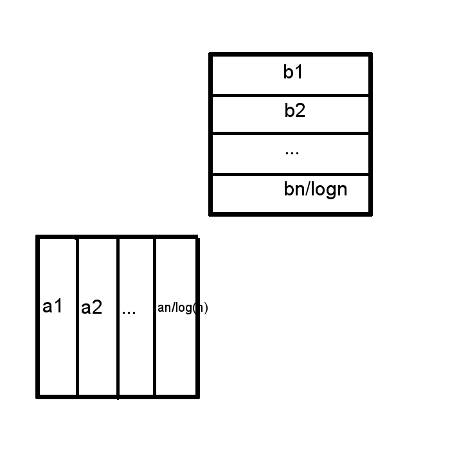
\includegraphics[scale=0.55]{images/17.png}

Liczymy iloczyny macierzy dla każdego $a_i \cdot b_i$. Takich iloczynów jest oczywiscie $\frac{n}{\log(n)}$, 
a każdy w wyniku daje jedną macierz kwadratową. Jeśli zsumujemy te macierze to otrzymamy iloczyn, o który nam chodzi.

%%%%%%%%%%%%%%%%%%%%%%%%%%%
\section{}
\begin{framed}
Opisz, w jaki sposób DFS może być zastosowane do znalezienia cyklu Eulera w grafie.
\end{framed}

Graf przechodzimy przy pomocy rekurencyjnej procedury DFS. Przebyte krawędzie usuwamy, a wierzchołki po zakończeniu przetwarzania umieszczamy na początku kolejki. Jeśli graf posiada cykl Eulera, to po zakończeniu algorytmu w kolejce znajdą się kolejne wierzchołki tego cyklu.


%%%%%%%%%%%%%%%%%%%%%%%%%%%
\section{??? tego chyba nie było jeszcze}
\begin{framed}
Narysuj sieć półczyszczacą o ośmiu wejściach.
\end{framed}

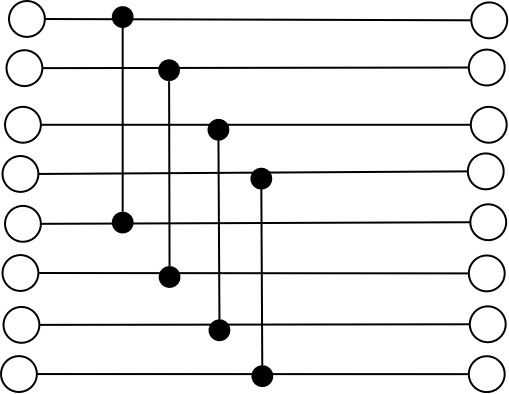
\includegraphics[scale=0.55]{images/20.png}

%%%%%%%%%%%%%%%%%%%%%%%%%%%
\section{??? tego chyba nie było jeszcze}
\begin{framed}
Narysuj automat rozpoznający $abaa$ i $abab$.
\end{framed}

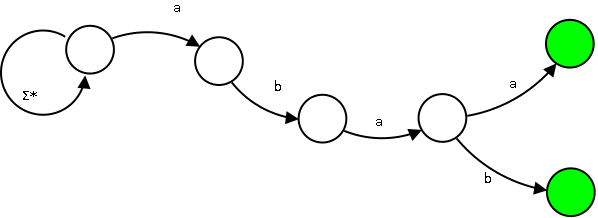
\includegraphics[scale=0.55]{images/22.png}

%%%%%%%%%%%%%%%%%%%%%%%%%%%
\section{}
\begin{framed}
W jaki sposób problem mnożenia macierzy może być wykorzystany do rozwiązania problemu najkrótszych ścieżek w grafie?
\end{framed}

Mamy grafy A i B w postaci macierzy adjacencji.\\
Możemy korzystać z algebry, w której:\\
'$+$' to działanie $\min$\\
'$\cdot$' to dodawanie\\
Wtedy jedno mnożenie macierzy, to jeden krok relaksacji najkrótszych ścieżek, musimy wykonać $n$ takich relaksacji. Złożoność $O(n^4)$. Można poprawić złożoność. Nie da się zastosować algorytmu Strassena, bo nie mamy działania odwrotnego do $\min$. Można za to skorzystać z szybkiego potęgowania, co zmniejsza nam koszt do $O(n^3\log n)$.

%%%%%%%%%%%%%%%%%%%%%%%%%%%
\section{}
\begin{framed}
Opisz, w jaki spósb obliczenie wielomianu n-tego stopnia w n-tych pierwiastkach jedności jest redukowalne do obliczenia dwóch wielomianów stopnia $n/2$ w $(n/2)$-tych pierwiastkach jedności.
\end{framed}

Mamy wielomian $A(x)$ stopnia $n$, reprezentowany przez współczynniki $a_0, a_1, \cdots, a_n$.\\
Tworzymy $2$ nowe wielomiany:\\
$A^{[0]}(x)=a_0 + a_2 x + a_4 x^2 + ... a_{n-2} x^{n/2 -1} + a_n x^{n/2}$\\
$A^{[1]}(x)=a_1 + a_3 x + a_5 x^2 + ... a_{n-1} x^{n/2 -1}$\\

$A(x) = A^{[0]}(x^2)+xA^{[1]}(x^2)$\\

\chapter{nierozwiązane}
%%%%%%%%%%%%%%%%%%%%%%%%%%%
\section{}
\begin{framed}
Opisz algrotym mnożenia długich liczb (n bitowych)?
\end{framed}

%%%%%%%%%%%%%%%%%%%%%%%%%%%
\section{} 
\begin{framed}
Jak posortwoać n liczb z przedziału $[1, n^2]$ w  czasie liniowym?
\end{framed}

%%%%%%%%%%%%%%%%%%%%%%%%%%%
\section{}
\begin{framed}
Ile warstw musi mieć siec przelączników, żeby dalo się uzyskać wszystkei przesunięcia cykliczne ciągu n-elemntowego?
\end{framed}
%%%%%%%%%%%%%%%%%%%%%%%%%%%%%%%%%%%%%%%%%%%%%%%%%%%%%%%%%%%%%%%%%%%%%%%%%%%%%%%%%%%%%%%%%%%%%%%%%%%%%

\begin{thebibliography}{99}
\end{thebibliography}
\end{document}



